\section{Pacemaker model}
\label{pacemakerModel}

Heart tissue can also be activated by external electrical pulses. 
\textsf{Implantable pacemakers} have been developed to deliver timely electrical pulses to the heart to maintain an appropriate heart rate and Atrial-Ventricular synchrony. 
Implantable pacemakers normally have two leads fixed on the wall of the right atrium and the right ventricle respectively (\ref{conduction} (a)). 
These leads are capable of both sensing electrical activity in the heart tissue, and of emitting pacing signals into the tissue. 
Tissue activation near the leads is sensed by the leads, triggering Atrial Sense ($A_{sense}$) and Ventricular Sense ($V_{sense}$) events in the pacemaker (see \ref{conduction} (b)). 
Atrial Pacing (AP) and Ventricular Pacing (VP) are delivered if no sensed events occur within pre-specified deadlines. Because a (dual chamber) pacemaker only utilizes activation timing information for two small regions in the heart, its limited knowledge of the current heart condition could lead to potential incorrect estimation of the heart's electrical activity and result in inappropriate therapies.

In order to deal with different heart conditions, modern pacemakers can be programmed to operate in different modes. The modes are labeled using a three character system (e.g. DDD) by the Heart Rhythm Society \cite{fogoros}. The first character describes the pacing locations (i.e. atrium or ventricle or both), the second character describes the sensing locations, and the third character describes how the pacemaker software responds to sensing. For example, the dual-chamber DDD mode stands for sensing in both atrium and ventricle, and pacing both of them if needed. In this effort, we describe two of the most commonly used modes of pacemaker, the dual-chamber DDD mode, that paces both the atrium and the ventricle, senses both chambers, and sensing can both activate or inhibit further pacing. Similarly, the VDI mode paces only in the ventricle, senses both chambers, and inhibits pacing if event is sensed \cite{pacemaker}. During certain heart condition changes, the pacemaker has to switch between different modes to achieve better treatment. It is very important to ensure that the mode-switches are performed as intended, and no safety issues can occur during the transition between different modes.

The coordinated contraction of the atria and the ventricles are governed by the electrical conduction system of the heart (\ref{conduction}). Despite the varieties of the cells, cells in the heart generate \emph{action potential} when an electrical potential is applied to them (\ref{act_pot}), and their action potentials share similar properties. The action potential can be divided into: \emph{Rest} period during which a new and normal action potential can be initialized, either by potential difference applied to the cell or by itself for pacemaker cells; \emph{Effective Refractory Period} (ERP) which is initialized by the depolarization of the cell, and during which no new action potential can be initialized; \emph{Relative Refractory Period} (RRP) during which a new but abnormal action potential can be initialized. In the VHM this behavior is captured using \textbf{node automaton} (\ref{node}). The timing periods described above are modeled as states with corresponding timers. 

%%%%%%%%%%%%%%%%%%%%%%%%%%%%%%%%%%%%%%%%%%%%%%
\begin{figure*}[!t]
	\centering
	\vspace{-10pt}
	\subfigure [\small]{
		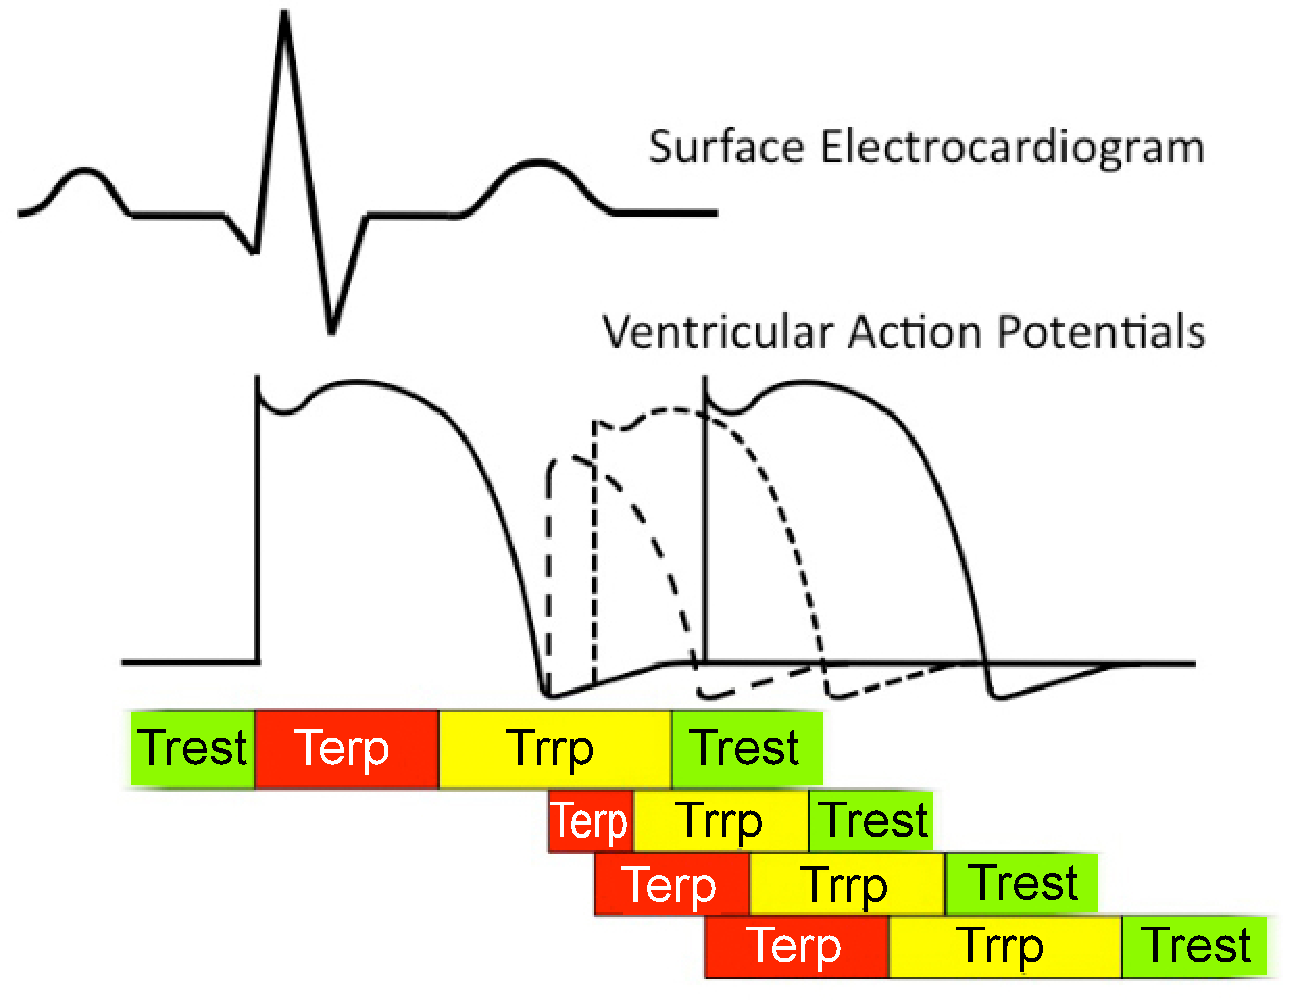
\includegraphics[width=0.3\textwidth]{figures/act_pot_new.pdf}
		\label{fig:act_pot}
	} 
	\subfigure [\small] 
	{	
		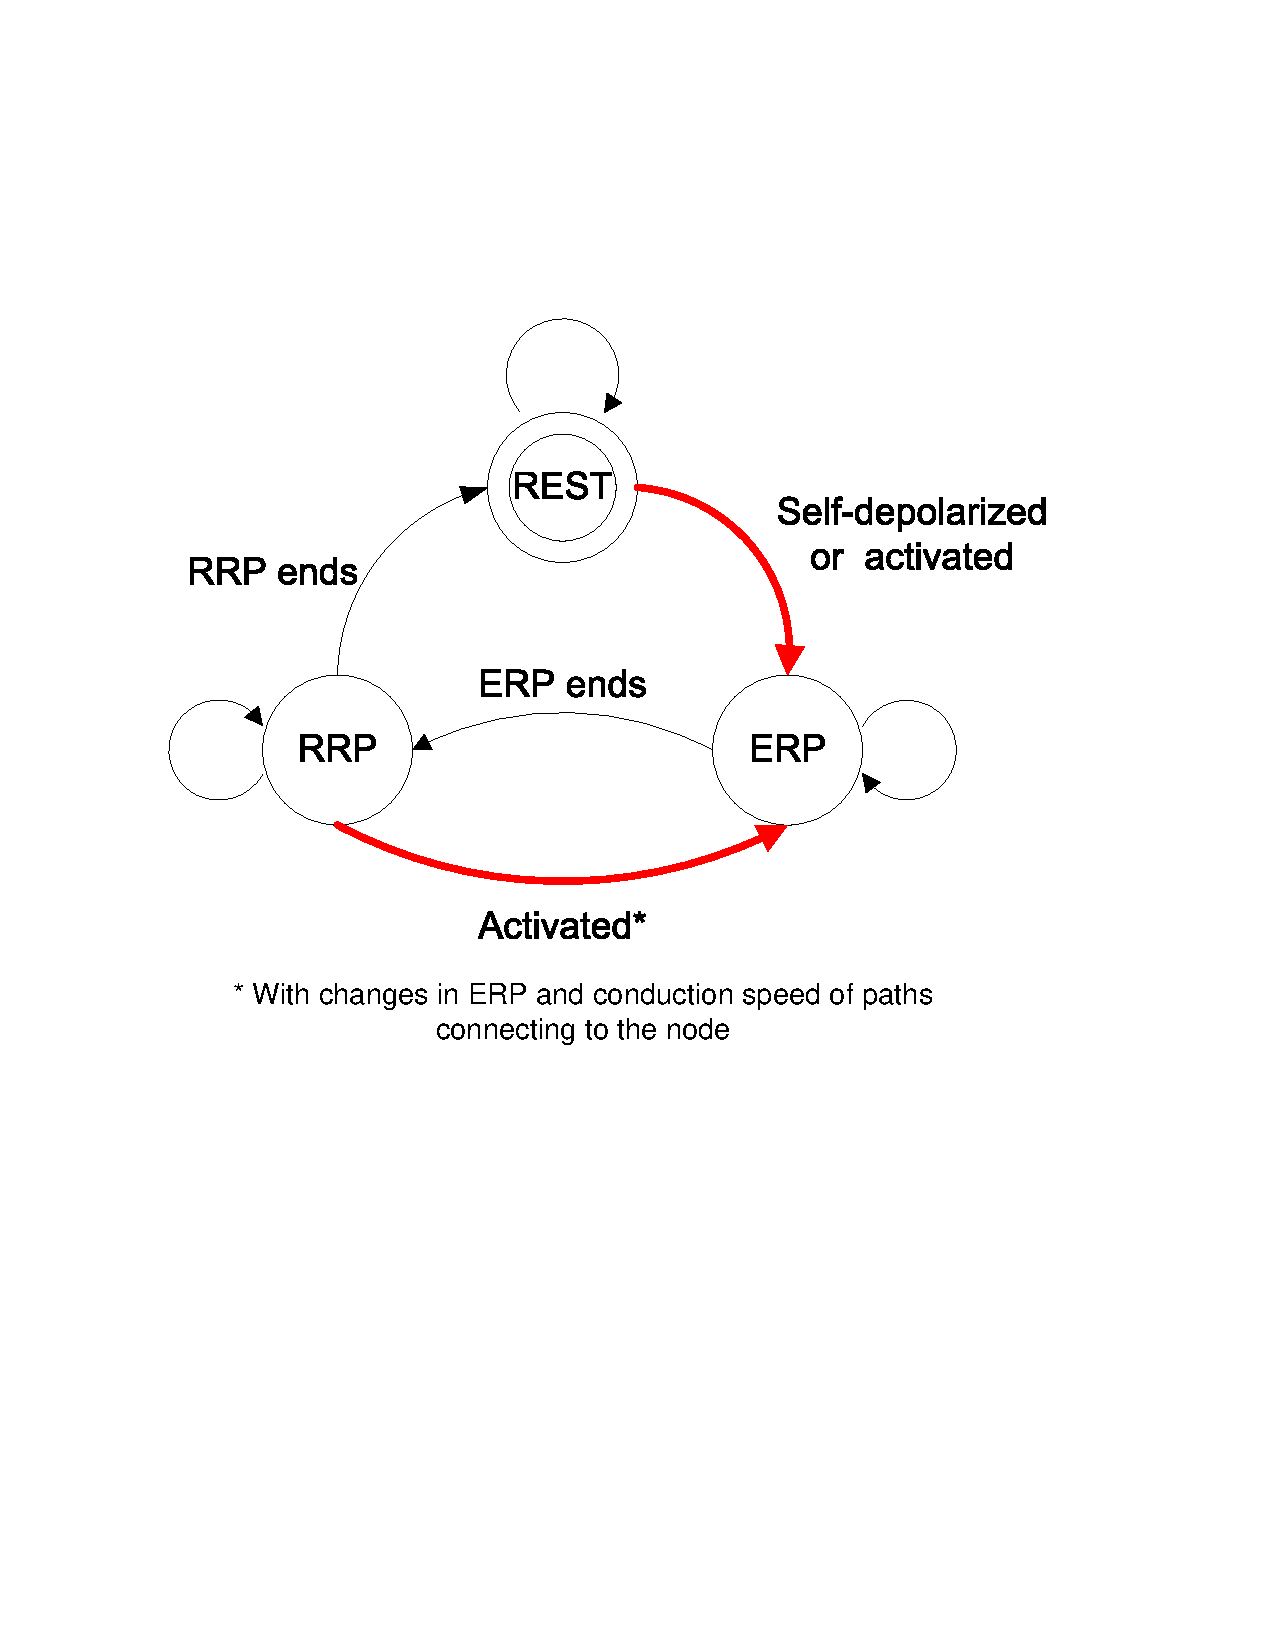
\includegraphics[width=0.27\textwidth]{figures/node_automata.pdf}
		\label{fig:node}
	}
	\subfigure [\small] 
	{
		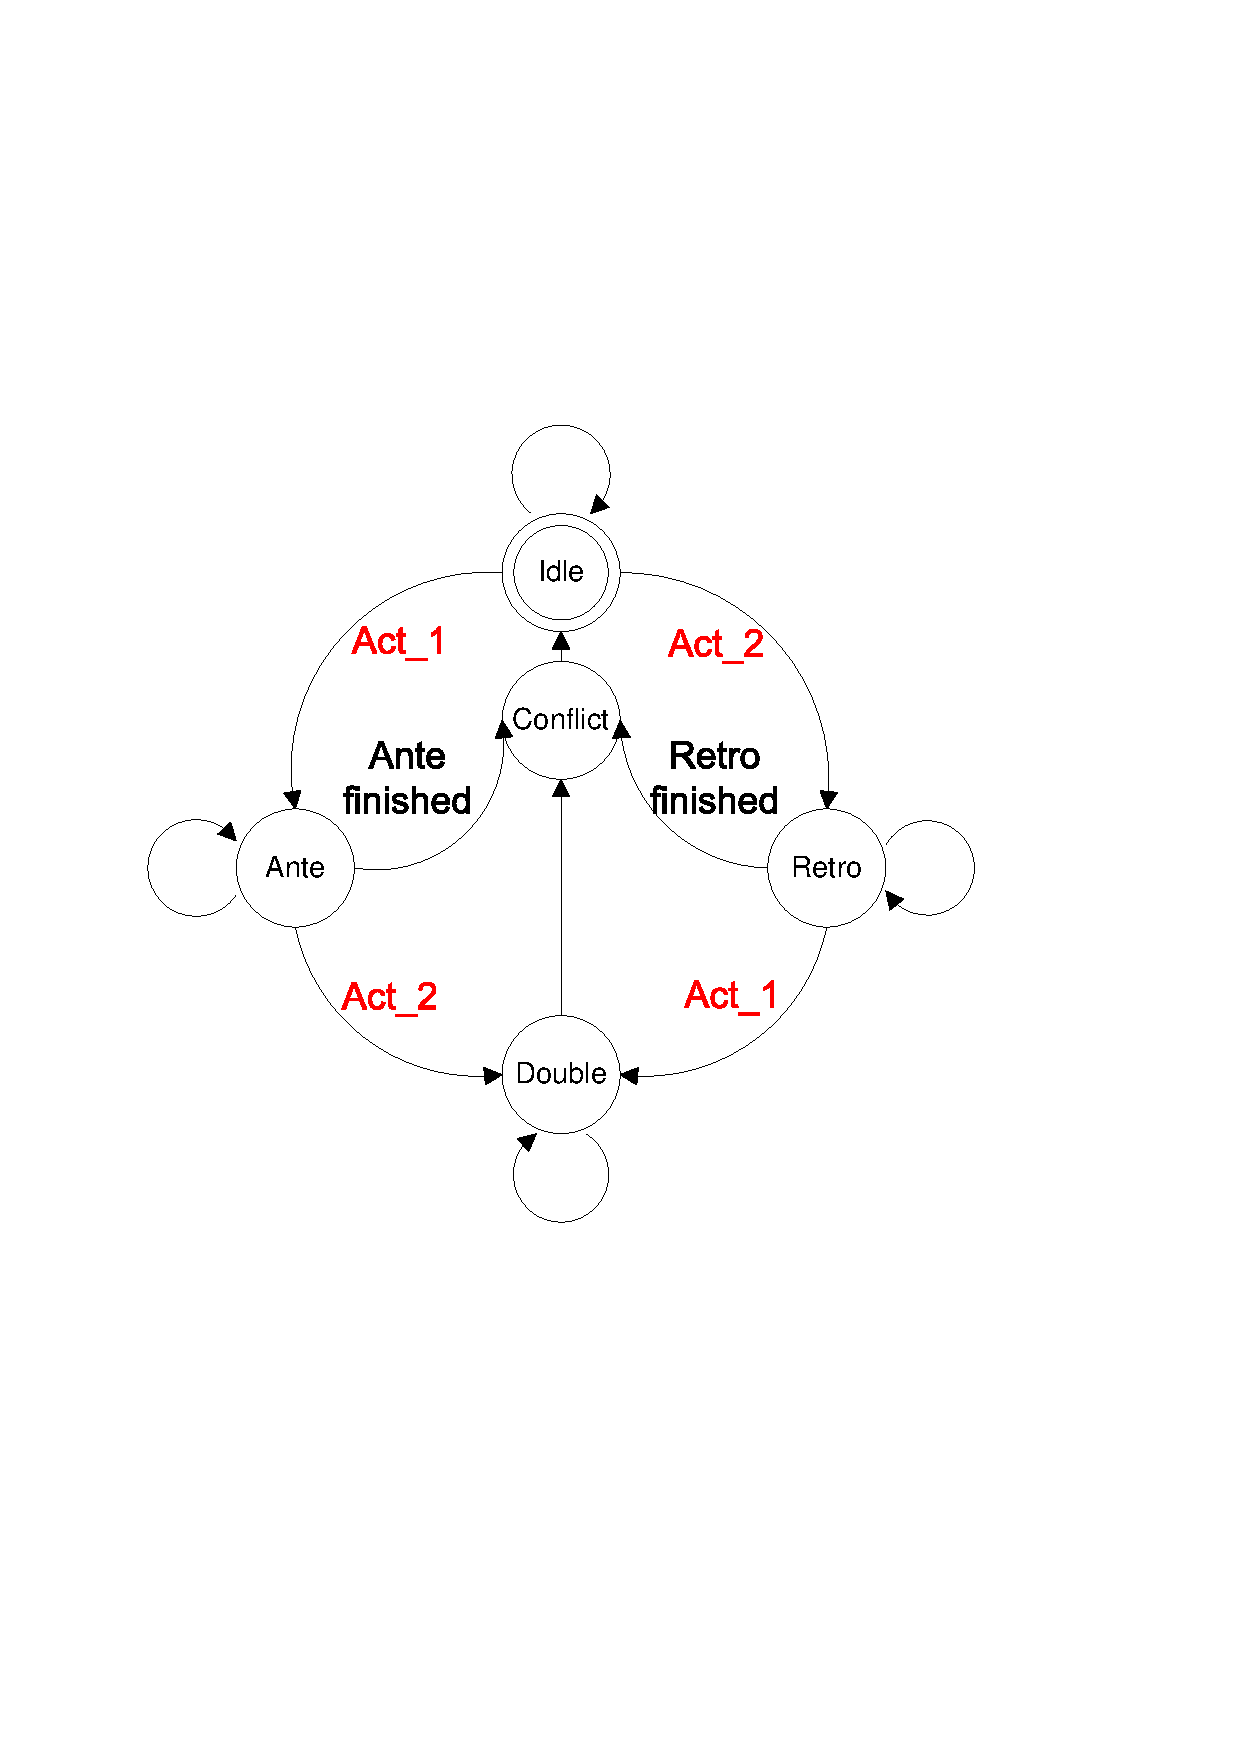
\includegraphics[width=0.27\textwidth]{figures/path_automata.pdf}
		\label{fig:path}
	} 
	\label{fig:h_automatas}
	\vspace{-8pt}
	\caption{\small (a) Action potential recorded from ventricular tissue. The dashed lines show how action potential morphology changes when a stimulus is applied early to the tissue and how the corresponding timer values change.(b) Node automaton. (c) Path automaton}
	\vspace{-10pt}
\end{figure*} 
%%%%%%%%%%%%%%%%%%%%%%%%%%%%%%%%%%%%%%%%%%%%%%

The electrical potential difference caused by the depolarization of one cell can trigger depolarization of the cells nearby. This propagation property is captured using \textbf{path automaton} (\ref{path}). So the electrical conduction system of the heart can be represented as conduction pathways. Since the refractory properties along a conduction pathway are governed by the tissue at both ends of the path \cite{josephson}, one conduction pathway can be represented as two node automata connected by a path automata. The electrical conduction system of the heart represented using node and path automata is shown in \ref{general_setup}. The timing properties of the system are modeled by the timed automata and the spatial properties of the system is kept by overlaying the automata onto a 2-D heart anatomy. The VHM is implemented in Simulink. We were able to use VHM to simulate different heart conditions in a closed-loop with the pacemaker model. Some representative heart conditions including (1) Wenckebach AV nodal response, (2) AV Nodal Reentry Tachycardia (AVNRT), (3) Atrial Flutter (AF), (4) Pacemaker mode-switch operation and (5) Pacemaker mediated tachycardia.

The VHM誷 functional output has been validated by the director of cardiac electrophysiology in the Philadelphia VA Hospital and by electrophysiologists in the Hospital of the University of Pennsylvania. The model generates outputs (Electrograms) which matches the output of a real heart with same underlying heart condition when inputs (Programmed pacing) are applied to it. More detailed description of node and path automaton implementation and case studies can be found in our previous papers \cite{Jiang1}\cite{vhm_iccps11}\cite{embc10}.

\section{Pacemaker model}

In order to show the capability of VHM in Implantable Cardiac Device Validation \& Verification, a simple pacemaker model is developed. Pacemakers operate in different modes and these are labeled using a three character system (e.g. xyz). The first position describes the pacing locations, the second location describes the sensing locations, and the third position describes how the pacemaker software responds to sensing. For example, the DDD mode paces both the atrium and ventricle (D), senses both (D), and sensing can both activate or inhibit further pacing (D). We developed a basic DDD pacemaker model according to  to the specification derived from \cite{challenge}.\\
\textbf{1. Lower Rate Interval (LRI)}:
The LRI interval starts at a ventricular sensed or paced event. The LRI interval is the longest interval between two ventricular events. 

\textbf{2. Upper Rate Interval (URI)}:
The URI interval defines the shortest interval between a ventricular event and a paced ventricular event

\textbf{3. Atrial-Ventricular Interval (AVI)}:
Ventricular pacing shall occur in the absence of a sensed ventricular event within the programmed AV delay when the time elapsed after the last ventricular event is between the programmed LRI and URI.

\textbf{4. Ventricular Refractory Period (VRP)}:
The VRP is the time interval following a ventricular event during which no ventricular sense (VS) can happen.

\textbf{5. Post Ventricular Atrial Refractory Period (PVARP)}:
The PVARP is the time interval following a ventricular event during which no atrial sense (AS) can happen.

According to the five primary specifications of the basic DDD pacemaker, a Simulink model was designed using temporal logic. Each component corresponds to a particular specification and communicates with others using channels. A timing diagram is shown in \ref{timingPM}. This model can be easily translated into formal verification tool called UPPAAL for timing verification. More information about the implementation can be found in \cite{STTT13}. 

%%%%%%%%%%%%%%%%%%%%%%%%%%%%%%%%%%%%%%%%%%%%%%
\begin{figure}[!b]
	\center
	\vspace{-10pt}
	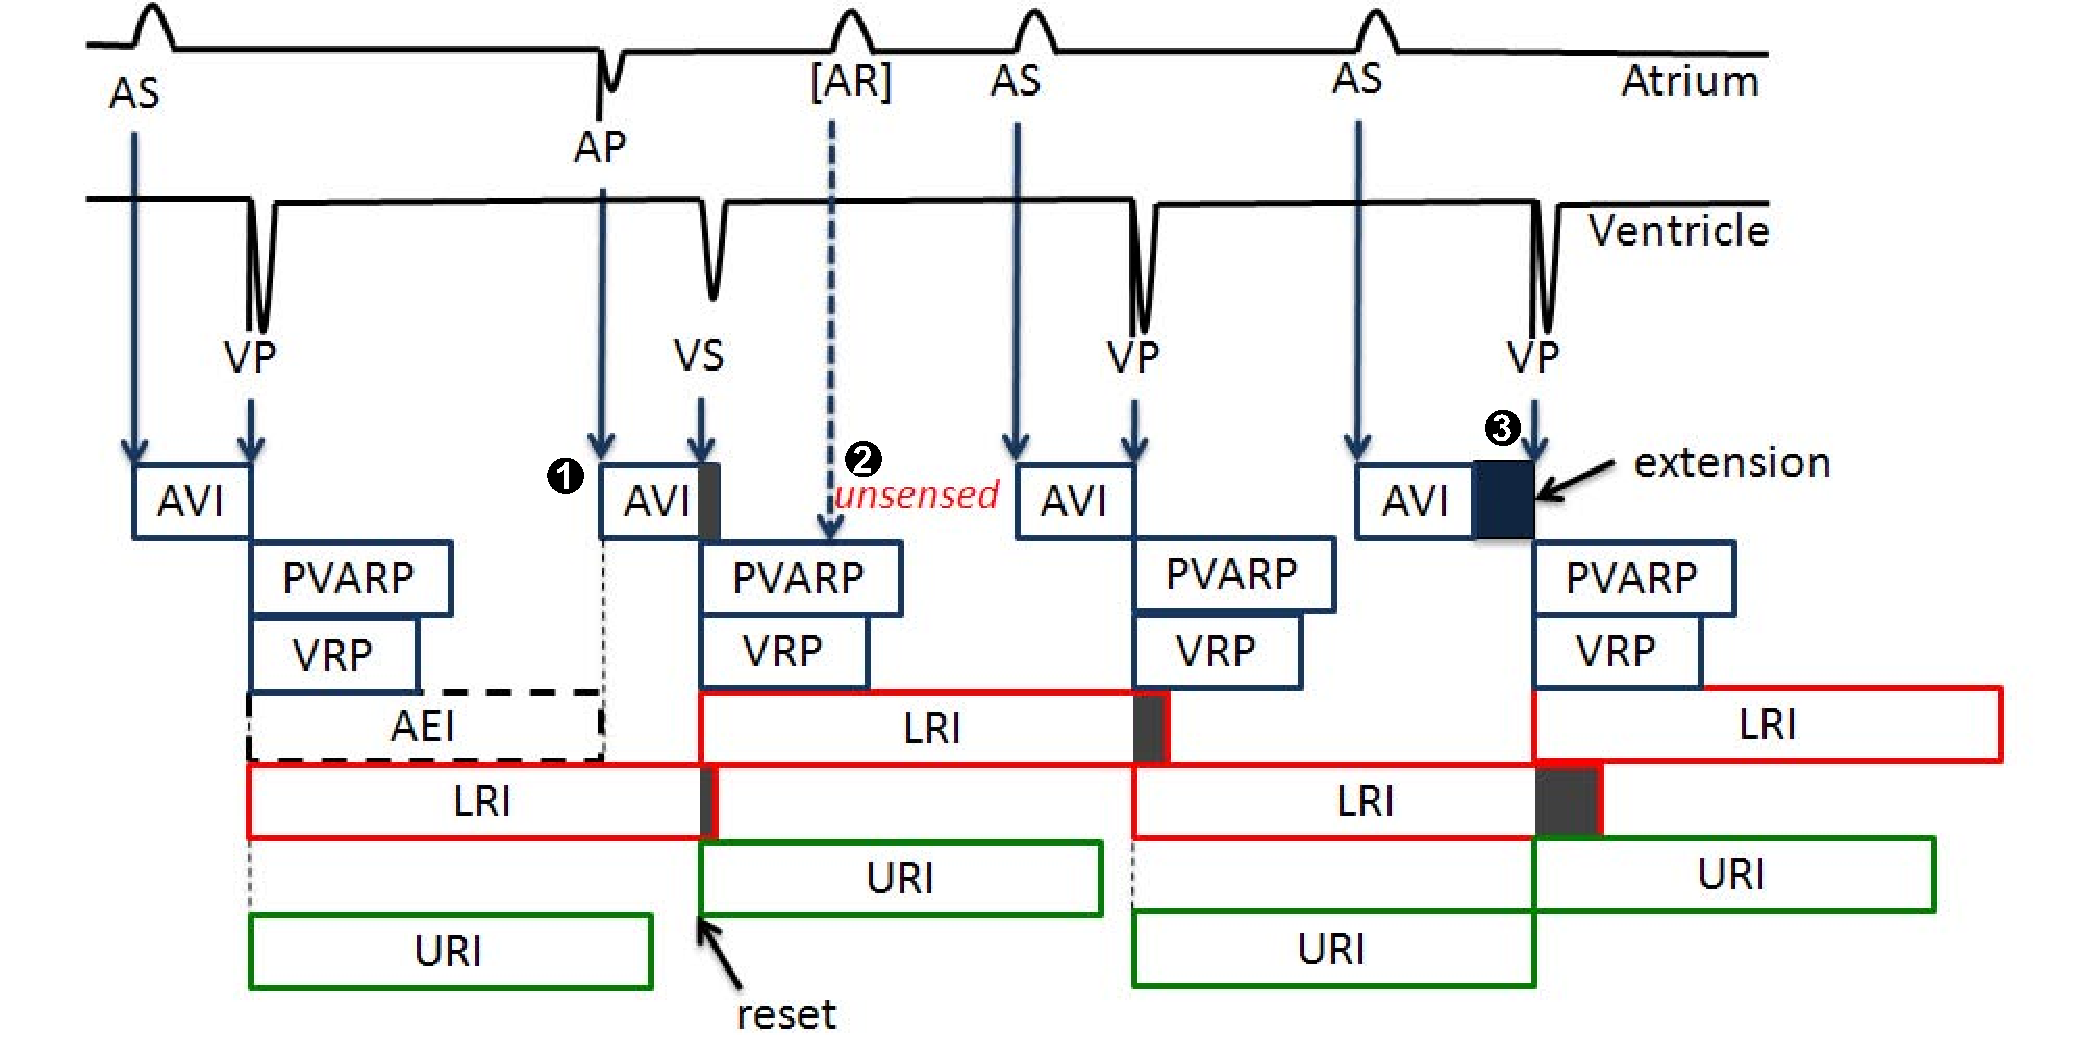
\includegraphics[width=0.45\textwidth]{figures/PM_timers.pdf}
	\vspace{-10pt}
	\caption{Simulink design of path automata}
	\label{fig:timingPM}
\end{figure}